\documentclass[twoside]{book}

% Packages required by doxygen
\usepackage{fixltx2e}
\usepackage{calc}
\usepackage{doxygen}
\usepackage[export]{adjustbox} % also loads graphicx
\usepackage{graphicx}
\usepackage[utf8]{inputenc}
\usepackage{makeidx}
\usepackage{multicol}
\usepackage{multirow}
\PassOptionsToPackage{warn}{textcomp}
\usepackage{textcomp}
\usepackage[nointegrals]{wasysym}
\usepackage[table]{xcolor}

% Font selection
\usepackage[T1]{fontenc}
\usepackage[scaled=.90]{helvet}
\usepackage{courier}
\usepackage{amssymb}
\usepackage{sectsty}
\renewcommand{\familydefault}{\sfdefault}
\allsectionsfont{%
  \fontseries{bc}\selectfont%
  \color{darkgray}%
}
\renewcommand{\DoxyLabelFont}{%
  \fontseries{bc}\selectfont%
  \color{darkgray}%
}
\newcommand{\+}{\discretionary{\mbox{\scriptsize$\hookleftarrow$}}{}{}}

% Page & text layout
\usepackage{geometry}
\geometry{%
  a4paper,%
  top=2.5cm,%
  bottom=2.5cm,%
  left=2.5cm,%
  right=2.5cm%
}
\tolerance=750
\hfuzz=15pt
\hbadness=750
\setlength{\emergencystretch}{15pt}
\setlength{\parindent}{0cm}
\setlength{\parskip}{0.2cm}
\makeatletter
\renewcommand{\paragraph}{%
  \@startsection{paragraph}{4}{0ex}{-1.0ex}{1.0ex}{%
    \normalfont\normalsize\bfseries\SS@parafont%
  }%
}
\renewcommand{\subparagraph}{%
  \@startsection{subparagraph}{5}{0ex}{-1.0ex}{1.0ex}{%
    \normalfont\normalsize\bfseries\SS@subparafont%
  }%
}
\makeatother

% Headers & footers
\usepackage{fancyhdr}
\pagestyle{fancyplain}
\fancyhead[LE]{\fancyplain{}{\bfseries\thepage}}
\fancyhead[CE]{\fancyplain{}{}}
\fancyhead[RE]{\fancyplain{}{\bfseries\leftmark}}
\fancyhead[LO]{\fancyplain{}{\bfseries\rightmark}}
\fancyhead[CO]{\fancyplain{}{}}
\fancyhead[RO]{\fancyplain{}{\bfseries\thepage}}
\fancyfoot[LE]{\fancyplain{}{}}
\fancyfoot[CE]{\fancyplain{}{}}
\fancyfoot[RE]{\fancyplain{}{\bfseries\scriptsize Generated on Wed Nov 11 2015 11\+:39\+:52 for i\+Ant-\/\+A\+R\+Go\+S by Doxygen }}
\fancyfoot[LO]{\fancyplain{}{\bfseries\scriptsize Generated on Wed Nov 11 2015 11\+:39\+:52 for i\+Ant-\/\+A\+R\+Go\+S by Doxygen }}
\fancyfoot[CO]{\fancyplain{}{}}
\fancyfoot[RO]{\fancyplain{}{}}
\renewcommand{\footrulewidth}{0.4pt}
\renewcommand{\chaptermark}[1]{%
  \markboth{#1}{}%
}
\renewcommand{\sectionmark}[1]{%
  \markright{\thesection\ #1}%
}

% Indices & bibliography
\usepackage{natbib}
\usepackage[titles]{tocloft}
\setcounter{tocdepth}{3}
\setcounter{secnumdepth}{5}
\makeindex

% Hyperlinks (required, but should be loaded last)
\usepackage{ifpdf}
\ifpdf
  \usepackage[pdftex,pagebackref=true]{hyperref}
\else
  \usepackage[ps2pdf,pagebackref=true]{hyperref}
\fi
\hypersetup{%
  colorlinks=true,%
  linkcolor=blue,%
  citecolor=blue,%
  unicode%
}

% Custom commands
\newcommand{\clearemptydoublepage}{%
  \newpage{\pagestyle{empty}\cleardoublepage}%
}


%===== C O N T E N T S =====

\begin{document}

% Titlepage & ToC
\hypersetup{pageanchor=false,
             bookmarks=true,
             bookmarksnumbered=true,
             pdfencoding=unicode
            }
\pagenumbering{roman}
\begin{titlepage}
\vspace*{7cm}
\begin{center}%
{\Large i\+Ant-\/\+A\+R\+Go\+S }\\
\vspace*{1cm}
{\large Generated by Doxygen 1.8.10}\\
\vspace*{0.5cm}
{\small Wed Nov 11 2015 11:39:52}\\
\end{center}
\end{titlepage}
\clearemptydoublepage
\tableofcontents
\clearemptydoublepage
\pagenumbering{arabic}
\hypersetup{pageanchor=true}

%--- Begin generated contents ---
\chapter{Hierarchical Index}
\section{Class Hierarchy}
This inheritance list is sorted roughly, but not completely, alphabetically\+:\begin{DoxyCompactList}
\item C\+C\+I\+\_\+\+Controller\begin{DoxyCompactList}
\item \contentsline{section}{i\+Ant\+Base\+Controller}{\pageref{classi_ant_base_controller}}{}
\begin{DoxyCompactList}
\item \contentsline{section}{C\+P\+F\+A\+\_\+controller}{\pageref{class_c_p_f_a__controller}}{}
\item \contentsline{section}{D\+S\+A\+\_\+controller}{\pageref{class_d_s_a__controller}}{}
\end{DoxyCompactList}
\end{DoxyCompactList}
\item C\+Loop\+Functions\begin{DoxyCompactList}
\item \contentsline{section}{C\+P\+F\+A\+\_\+loop\+\_\+functions}{\pageref{class_c_p_f_a__loop__functions}}{}
\item \contentsline{section}{i\+Ant\+Base\+Controller}{\pageref{classi_ant_base_controller}}{}
\end{DoxyCompactList}
\item \contentsline{section}{D\+S\+A\+\_\+loop\+\_\+functions}{\pageref{class_d_s_a__loop__functions}}{}
\item \contentsline{section}{i\+Ant\+Food}{\pageref{classi_ant_food}}{}
\item \contentsline{section}{i\+Ant\+Pheromone}{\pageref{classi_ant_pheromone}}{}
\end{DoxyCompactList}

\chapter{Class Index}
\section{Class List}
Here are the classes, structs, unions and interfaces with brief descriptions\+:\begin{DoxyCompactList}
\item\contentsline{section}{\hyperlink{class_c_p_f_a__controller}{C\+P\+F\+A\+\_\+controller} }{\pageref{class_c_p_f_a__controller}}{}
\item\contentsline{section}{\hyperlink{class_c_p_f_a__loop__functions}{C\+P\+F\+A\+\_\+loop\+\_\+functions} }{\pageref{class_c_p_f_a__loop__functions}}{}
\item\contentsline{section}{\hyperlink{class_d_s_a__controller}{D\+S\+A\+\_\+controller} }{\pageref{class_d_s_a__controller}}{}
\item\contentsline{section}{\hyperlink{class_d_s_a__loop__functions}{D\+S\+A\+\_\+loop\+\_\+functions} }{\pageref{class_d_s_a__loop__functions}}{}
\item\contentsline{section}{\hyperlink{classi_ant_base_controller}{i\+Ant\+Base\+Controller} }{\pageref{classi_ant_base_controller}}{}
\item\contentsline{section}{\hyperlink{classi_ant_food}{i\+Ant\+Food} }{\pageref{classi_ant_food}}{}
\item\contentsline{section}{\hyperlink{classi_ant_pheromone}{i\+Ant\+Pheromone} }{\pageref{classi_ant_pheromone}}{}
\end{DoxyCompactList}

\chapter{Class Documentation}
\hypertarget{class_c_p_f_a__controller}{}\section{C\+P\+F\+A\+\_\+controller Class Reference}
\label{class_c_p_f_a__controller}\index{C\+P\+F\+A\+\_\+controller@{C\+P\+F\+A\+\_\+controller}}
Inheritance diagram for C\+P\+F\+A\+\_\+controller\+:\begin{figure}[H]
\begin{center}
\leavevmode
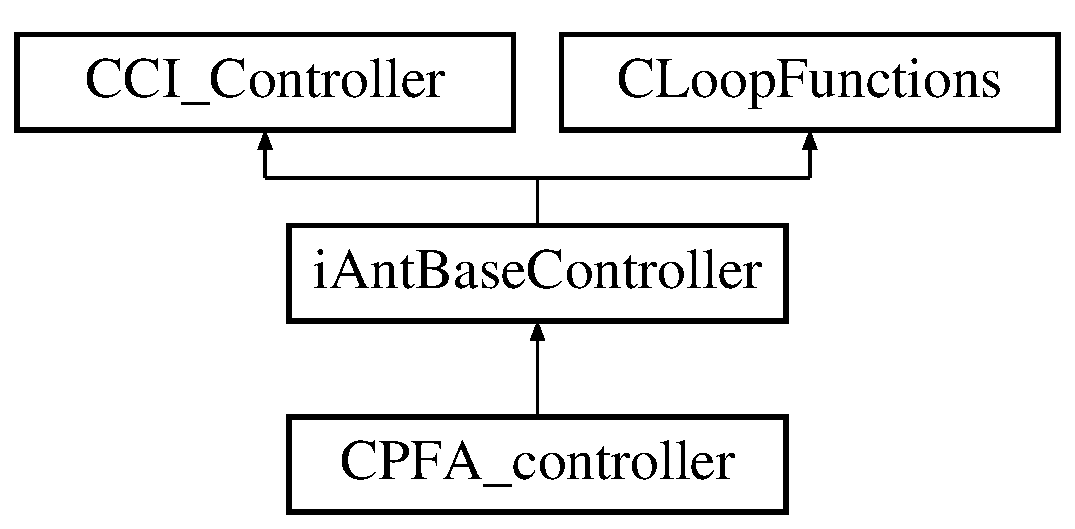
\includegraphics[height=3.000000cm]{class_c_p_f_a__controller}
\end{center}
\end{figure}
\subsection*{Public Member Functions}
\begin{DoxyCompactItemize}
\item 
\hypertarget{class_c_p_f_a__controller_af533ecc405586f4f8c9acc05907bffad}{}void {\bfseries Init} (argos\+::\+T\+Configuration\+Node \&t\+\_\+node)\label{class_c_p_f_a__controller_af533ecc405586f4f8c9acc05907bffad}

\item 
\hypertarget{class_c_p_f_a__controller_a553ca573fb8bb5aca7bec2adba20be71}{}void {\bfseries Control\+Step} ()\label{class_c_p_f_a__controller_a553ca573fb8bb5aca7bec2adba20be71}

\item 
\hypertarget{class_c_p_f_a__controller_a3049b8dd12ffc4e6cd44ba6046d73708}{}void {\bfseries Reset} ()\label{class_c_p_f_a__controller_a3049b8dd12ffc4e6cd44ba6046d73708}

\end{DoxyCompactItemize}
\subsection*{Additional Inherited Members}


The documentation for this class was generated from the following files\+:\begin{DoxyCompactItemize}
\item 
source/\+C\+P\+F\+A/C\+P\+F\+A\+\_\+controller.\+h\item 
source/\+C\+P\+F\+A/C\+P\+F\+A\+\_\+controller.\+cpp\end{DoxyCompactItemize}

\hypertarget{class_c_p_f_a__loop__functions}{}\section{C\+P\+F\+A\+\_\+loop\+\_\+functions Class Reference}
\label{class_c_p_f_a__loop__functions}\index{C\+P\+F\+A\+\_\+loop\+\_\+functions@{C\+P\+F\+A\+\_\+loop\+\_\+functions}}
Inheritance diagram for C\+P\+F\+A\+\_\+loop\+\_\+functions\+:\begin{figure}[H]
\begin{center}
\leavevmode
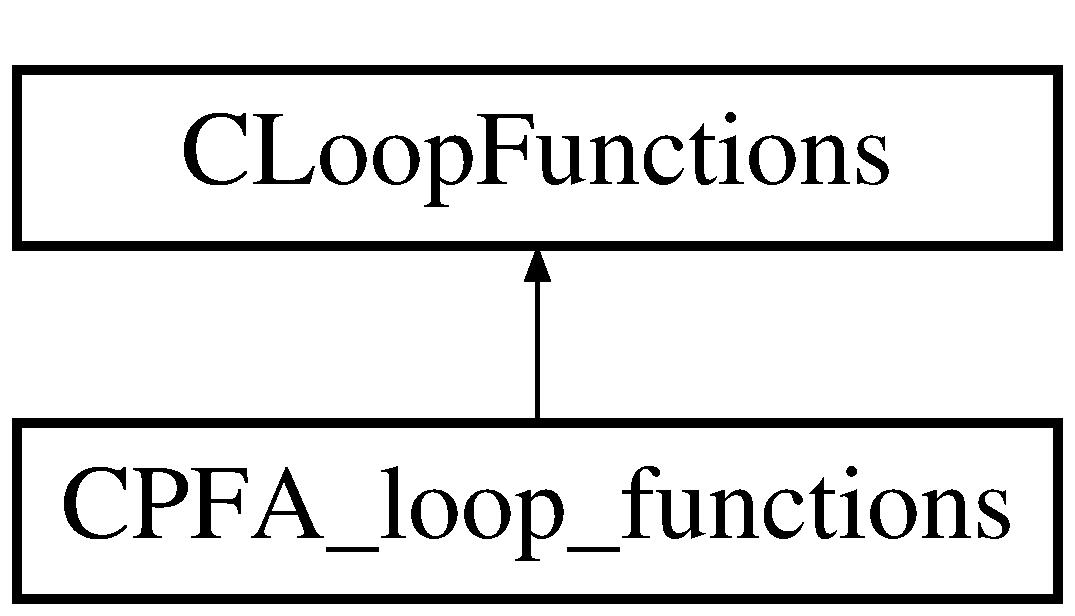
\includegraphics[height=2.000000cm]{class_c_p_f_a__loop__functions}
\end{center}
\end{figure}
\subsection*{Public Member Functions}
\begin{DoxyCompactItemize}
\item 
\hypertarget{class_c_p_f_a__loop__functions_a97f6f1c4ac27f57f9d318d30f38ef1b9}{}void {\bfseries Init} (argos\+::\+T\+Configuration\+Node \&t\+\_\+tree)\label{class_c_p_f_a__loop__functions_a97f6f1c4ac27f57f9d318d30f38ef1b9}

\item 
\hypertarget{class_c_p_f_a__loop__functions_ac905a10128796e0bc1d2e7d8e5842dff}{}void {\bfseries Reset} ()\label{class_c_p_f_a__loop__functions_ac905a10128796e0bc1d2e7d8e5842dff}

\item 
\hypertarget{class_c_p_f_a__loop__functions_addb33071e767b219404c551f164c0445}{}void {\bfseries Destroy} ()\label{class_c_p_f_a__loop__functions_addb33071e767b219404c551f164c0445}

\item 
\hypertarget{class_c_p_f_a__loop__functions_a3495b36545b53118cc336be9e954a3ce}{}void {\bfseries Pre\+Step} ()\label{class_c_p_f_a__loop__functions_a3495b36545b53118cc336be9e954a3ce}

\item 
\hypertarget{class_c_p_f_a__loop__functions_a549dd30af6d26d0a080f801752a62e93}{}void {\bfseries Post\+Step} ()\label{class_c_p_f_a__loop__functions_a549dd30af6d26d0a080f801752a62e93}

\item 
\hypertarget{class_c_p_f_a__loop__functions_ad8fc7fe0e1b7c53c5071fa5745352c59}{}bool {\bfseries Is\+Experiment\+Finished} ()\label{class_c_p_f_a__loop__functions_ad8fc7fe0e1b7c53c5071fa5745352c59}

\item 
\hypertarget{class_c_p_f_a__loop__functions_a6841f721718a79cfca7866a9f010837f}{}void {\bfseries Post\+Experiment} ()\label{class_c_p_f_a__loop__functions_a6841f721718a79cfca7866a9f010837f}

\item 
\hypertarget{class_c_p_f_a__loop__functions_ae7dd1962bc63fe18ce9d27615154819a}{}argos\+::\+C\+Color {\bfseries Get\+Floor\+Color} (const argos\+::\+C\+Vector2 \&c\+\_\+pos\+\_\+on\+\_\+floor)\label{class_c_p_f_a__loop__functions_ae7dd1962bc63fe18ce9d27615154819a}

\end{DoxyCompactItemize}


The documentation for this class was generated from the following files\+:\begin{DoxyCompactItemize}
\item 
source/\+C\+P\+F\+A/C\+P\+F\+A\+\_\+loop\+\_\+functions.\+h\item 
source/\+C\+P\+F\+A/C\+P\+F\+A\+\_\+loop\+\_\+functions.\+cpp\end{DoxyCompactItemize}

\hypertarget{class_d_s_a__controller}{}\section{D\+S\+A\+\_\+controller Class Reference}
\label{class_d_s_a__controller}\index{D\+S\+A\+\_\+controller@{D\+S\+A\+\_\+controller}}
Inheritance diagram for D\+S\+A\+\_\+controller\+:\begin{figure}[H]
\begin{center}
\leavevmode
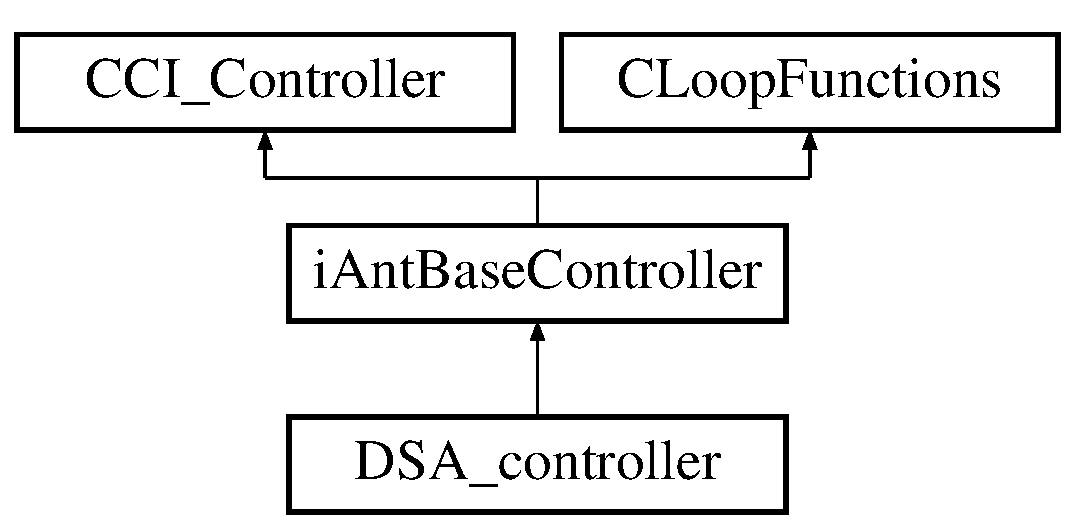
\includegraphics[height=3.000000cm]{class_d_s_a__controller}
\end{center}
\end{figure}
\subsection*{Public Member Functions}
\begin{DoxyCompactItemize}
\item 
\hypertarget{class_d_s_a__controller_a8891098013a4af1dcf7d5c8778387ff9}{}void {\bfseries Init} (argos\+::\+T\+Configuration\+Node \&t\+\_\+node)\label{class_d_s_a__controller_a8891098013a4af1dcf7d5c8778387ff9}

\item 
\hypertarget{class_d_s_a__controller_a5ac79d0e62322382799e9ad7834e4f4e}{}void {\bfseries Control\+Step} ()\label{class_d_s_a__controller_a5ac79d0e62322382799e9ad7834e4f4e}

\item 
\hypertarget{class_d_s_a__controller_aec7096f6666f694b5498b2d9dc424ff9}{}void {\bfseries Reset} ()\label{class_d_s_a__controller_aec7096f6666f694b5498b2d9dc424ff9}

\item 
\hypertarget{class_d_s_a__controller_a521abb258aba39cc9a3d7170001dfb78}{}void {\bfseries Destroy} ()\label{class_d_s_a__controller_a521abb258aba39cc9a3d7170001dfb78}

\end{DoxyCompactItemize}
\subsection*{Additional Inherited Members}


The documentation for this class was generated from the following file\+:\begin{DoxyCompactItemize}
\item 
source/\+D\+S\+A/D\+S\+A\+\_\+controller.\+h\end{DoxyCompactItemize}

\hypertarget{class_d_s_a__loop__functions}{}\section{D\+S\+A\+\_\+loop\+\_\+functions Class Reference}
\label{class_d_s_a__loop__functions}\index{D\+S\+A\+\_\+loop\+\_\+functions@{D\+S\+A\+\_\+loop\+\_\+functions}}


The documentation for this class was generated from the following file\+:\begin{DoxyCompactItemize}
\item 
source/\+D\+S\+A/D\+S\+A\+\_\+loop\+\_\+functions.\+h\end{DoxyCompactItemize}

\hypertarget{classi_ant_base_controller}{}\section{i\+Ant\+Base\+Controller Class Reference}
\label{classi_ant_base_controller}\index{i\+Ant\+Base\+Controller@{i\+Ant\+Base\+Controller}}


{\ttfamily \#include $<$i\+Ant\+Base\+Controller.\+h$>$}

Inheritance diagram for i\+Ant\+Base\+Controller\+:\begin{figure}[H]
\begin{center}
\leavevmode
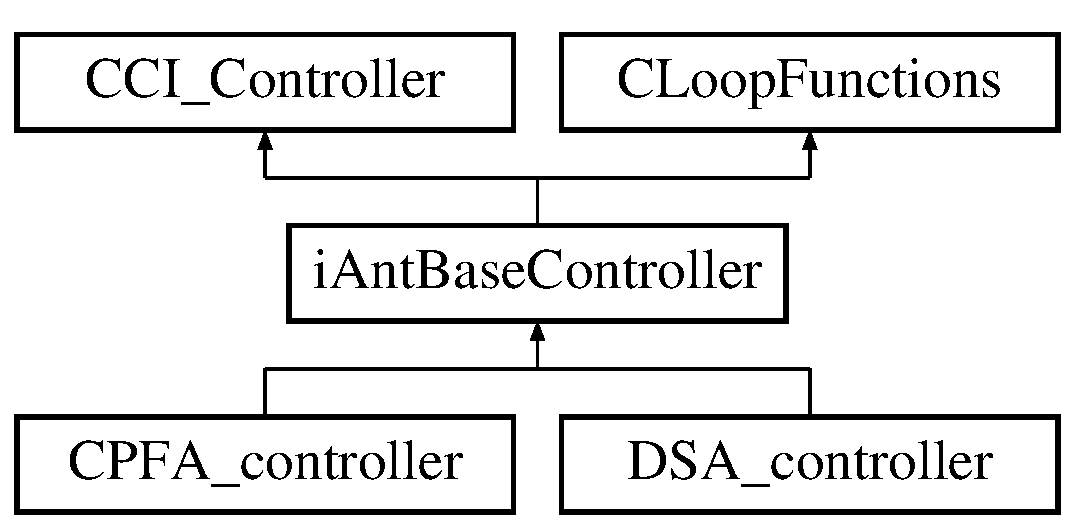
\includegraphics[height=3.000000cm]{classi_ant_base_controller}
\end{center}
\end{figure}
\subsection*{Public Member Functions}
\begin{DoxyCompactItemize}
\item 
\hyperlink{classi_ant_base_controller_a39d8d48963c82c29e7c943e431782d9a}{i\+Ant\+Base\+Controller} ()
\item 
\hypertarget{classi_ant_base_controller_ad42ec34c309ab33a650b7f28defc490e}{}argos\+::\+C\+Radians {\bfseries Get\+Heading} ()\label{classi_ant_base_controller_ad42ec34c309ab33a650b7f28defc490e}

\item 
\hypertarget{classi_ant_base_controller_aadadf8a3f8fbc5844428ec000a61ea6b}{}argos\+::\+C\+Vector2 {\bfseries Get\+Position} ()\label{classi_ant_base_controller_aadadf8a3f8fbc5844428ec000a61ea6b}

\item 
\hypertarget{classi_ant_base_controller_a27f63778f8fce4febcab7624f768cb0c}{}void {\bfseries Push\+Movement} (char move\+Type, argos\+::\+Real move\+Size)\label{classi_ant_base_controller_a27f63778f8fce4febcab7624f768cb0c}

\item 
\hypertarget{classi_ant_base_controller_a6e787198db6760b91130e3ec34038e1d}{}void {\bfseries Stop} ()\label{classi_ant_base_controller_a6e787198db6760b91130e3ec34038e1d}

\item 
\hypertarget{classi_ant_base_controller_af56e1a91b585793bcc877ee8b8f86d09}{}void {\bfseries Move} ()\label{classi_ant_base_controller_af56e1a91b585793bcc877ee8b8f86d09}

\item 
\hypertarget{classi_ant_base_controller_ac30e46e9048ce888af15fde012f9ba4e}{}size\+\_\+t {\bfseries Simulation\+Tick} ()\label{classi_ant_base_controller_ac30e46e9048ce888af15fde012f9ba4e}

\item 
\hypertarget{classi_ant_base_controller_aef393e9abb3037572f68f8c6884cfab3}{}size\+\_\+t {\bfseries Simulation\+Ticks\+Per\+Second} ()\label{classi_ant_base_controller_aef393e9abb3037572f68f8c6884cfab3}

\item 
\hypertarget{classi_ant_base_controller_a6a5c40fe9e57d61a50ff58abda6cda48}{}argos\+::\+Real {\bfseries Simulation\+Seconds\+Per\+Tick} ()\label{classi_ant_base_controller_a6a5c40fe9e57d61a50ff58abda6cda48}

\end{DoxyCompactItemize}
\subsection*{Protected Attributes}
\begin{DoxyCompactItemize}
\item 
\hypertarget{classi_ant_base_controller_aafc10e20b7821b436b531d6990b2a559}{}argos\+::\+Real {\bfseries Robot\+Forward\+Speed}\label{classi_ant_base_controller_aafc10e20b7821b436b531d6990b2a559}

\item 
\hypertarget{classi_ant_base_controller_a265916e97aa2ef53fdcc7ef55cc55392}{}argos\+::\+Real {\bfseries Robot\+Rotation\+Speed}\label{classi_ant_base_controller_a265916e97aa2ef53fdcc7ef55cc55392}

\item 
\hypertarget{classi_ant_base_controller_af7e0f181fc802153261874a2ac1215e8}{}argos\+::\+Real {\bfseries Target\+Travel\+Distance}\label{classi_ant_base_controller_af7e0f181fc802153261874a2ac1215e8}

\item 
\hypertarget{classi_ant_base_controller_abdc7a2a7dcc12dddc798ea7a0a4cdfb6}{}argos\+::\+Real {\bfseries Target\+Angle\+Distance}\label{classi_ant_base_controller_abdc7a2a7dcc12dddc798ea7a0a4cdfb6}

\item 
\hypertarget{classi_ant_base_controller_af501676396763245c6dfb72888b279f4}{}argos\+::\+Real {\bfseries Ticks\+To\+Wait}\label{classi_ant_base_controller_af501676396763245c6dfb72888b279f4}

\item 
\hypertarget{classi_ant_base_controller_a8de3da5a56a5bc97aa79999bab12ecdd}{}argos\+::\+C\+C\+I\+\_\+\+Positioning\+Sensor $\ast$ {\bfseries compass\+Sensor}\label{classi_ant_base_controller_a8de3da5a56a5bc97aa79999bab12ecdd}

\item 
\hypertarget{classi_ant_base_controller_a7491fc4f9773de742e874c5708395c7d}{}argos\+::\+C\+C\+I\+\_\+\+Differential\+Steering\+Actuator $\ast$ {\bfseries wheel\+Actuator}\label{classi_ant_base_controller_a7491fc4f9773de742e874c5708395c7d}

\item 
\hypertarget{classi_ant_base_controller_ab7f6d73f7a5e97a16a637e227a90806f}{}argos\+::\+C\+C\+I\+\_\+\+Foot\+Bot\+Proximity\+Sensor $\ast$ {\bfseries proximity\+Sensor}\label{classi_ant_base_controller_ab7f6d73f7a5e97a16a637e227a90806f}

\end{DoxyCompactItemize}


\subsection{Detailed Description}
\hyperlink{classi_ant_base_controller}{i\+Ant\+Base\+Controller} \begin{DoxyAuthor}{Author}
Antonio Griego 
\end{DoxyAuthor}


\subsection{Constructor \& Destructor Documentation}
\hypertarget{classi_ant_base_controller_a39d8d48963c82c29e7c943e431782d9a}{}\index{i\+Ant\+Base\+Controller@{i\+Ant\+Base\+Controller}!i\+Ant\+Base\+Controller@{i\+Ant\+Base\+Controller}}
\index{i\+Ant\+Base\+Controller@{i\+Ant\+Base\+Controller}!i\+Ant\+Base\+Controller@{i\+Ant\+Base\+Controller}}
\subsubsection[{i\+Ant\+Base\+Controller()}]{\setlength{\rightskip}{0pt plus 5cm}i\+Ant\+Base\+Controller\+::i\+Ant\+Base\+Controller (
\begin{DoxyParamCaption}
{}
\end{DoxyParamCaption}
)}\label{classi_ant_base_controller_a39d8d48963c82c29e7c943e431782d9a}
Constructor for the \hyperlink{classi_ant_base_controller}{i\+Ant\+Base\+Controller}. Several important variables are defined here. 

T\+O\+D\+O\+: update xml configuration file to allow these to be adjusted from configuration without recompiling. 

The documentation for this class was generated from the following files\+:\begin{DoxyCompactItemize}
\item 
source/i\+Ant\+Base/i\+Ant\+Base\+Controller.\+h\item 
source/i\+Ant\+Base/i\+Ant\+Base\+Controller.\+cpp\end{DoxyCompactItemize}

\hypertarget{classi_ant_food}{}\section{i\+Ant\+Food Class Reference}
\label{classi_ant_food}\index{i\+Ant\+Food@{i\+Ant\+Food}}


The documentation for this class was generated from the following file\+:\begin{DoxyCompactItemize}
\item 
source/i\+Ant\+Base/i\+Ant\+Food.\+h\end{DoxyCompactItemize}

\hypertarget{classi_ant_pheromone}{}\section{i\+Ant\+Pheromone Class Reference}
\label{classi_ant_pheromone}\index{i\+Ant\+Pheromone@{i\+Ant\+Pheromone}}


The documentation for this class was generated from the following file\+:\begin{DoxyCompactItemize}
\item 
source/i\+Ant\+Base/i\+Ant\+Pheromone.\+h\end{DoxyCompactItemize}

%--- End generated contents ---

% Index
\backmatter
\newpage
\phantomsection
\clearemptydoublepage
\addcontentsline{toc}{chapter}{Index}
\printindex

\end{document}
